%% -*- TeX-engine: luatex; ispell-language: russian -*-

\documentclass[a4paper,12pt]{article}

\usepackage[left=1.5cm,right=2cm,top=1.5cm,bottom=2cm]{geometry}

\usepackage{parskip}
\setlength{\parindent}{0mm}
\setcounter{secnumdepth}{1}

\usepackage{amsmath}

\usepackage{fontspec}
\setmainfont{PT Serif}
\newfontfamily\cyrillicfont[Script=Cyrillic,Ligatures=TeX]{PT Serif}
\setsansfont{PT Sans}
\setmonofont[Ligatures=NoCommon]{PT Mono}
\defaultfontfeatures{Ligatures=TeX}

\usepackage[bold-style=ISO]{unicode-math}
\setmathfont{XITS Math}

\usepackage{microtype}

\usepackage{hyperref}

\usepackage{polyglossia}
\setmainlanguage{russian}
\setotherlanguage{english}

\usepackage{csquotes}

%% for code snippets
\usepackage{minted}
\newminted[pycon]{pycon}{fontsize=\footnotesize}
\newminted[python3]{python3}{fontsize=\footnotesize}
\newminted[bash]{bash}{fontsize=\footnotesize}
\newmintinline[pythoninline]{python3}{fontsize=\footnotesize}
\newmintinline[bashinline]{bash}{fontsize=\footnotesize}

\pagestyle{empty}


\usepackage{blkarray}
\newcommand{\matindex}[1]{\mbox{\scriptsize#1}}

\usepackage{multicol}

\begin{document}
  \subsection*{Тест №3\hfill{15 марта 2017}}

  \makebox[\textwidth]{Представьтесь:\enspace\hrulefill}
  \paragraph{1} Какие проблемы могут возникнуть при использовании метода k-means? Как их избежать?

  \makebox[\linewidth]{\hrulefill}
  \makebox[\linewidth]{\hrulefill}
  \makebox[\linewidth]{\hrulefill}
  \makebox[\linewidth]{\hrulefill}

	\paragraph{2} Каким образом выбираются центры кластеров в алгоритме k-means++?
	
  \makebox[\linewidth]{\hrulefill}
  \makebox[\linewidth]{\hrulefill}
  \makebox[\linewidth]{\hrulefill}
	
  \paragraph{3}  Приведите пример кластерной структуры на которой алгоритм
  Ланса-Уильямса с параметрами, соответствующими групповому среднему, будет
  работать плохо.

  \hspace{6em}
  
  \paragraph{4} Что такое отступ обобщенного метрического классификатора?

  \makebox[\linewidth]{\hrulefill}
  \makebox[\linewidth]{\hrulefill}

  \paragraph{5} 
  \begin{minipage}{0.45\linewidth}
    Посмотрите на дендрограмму. Что отложено на горизонтальной оси? Какой смысл имеет длина ветвей дендрограммы? \\     
  \end{minipage}%  
  \begin{minipage}{0.45\linewidth}
    \begin{center}
      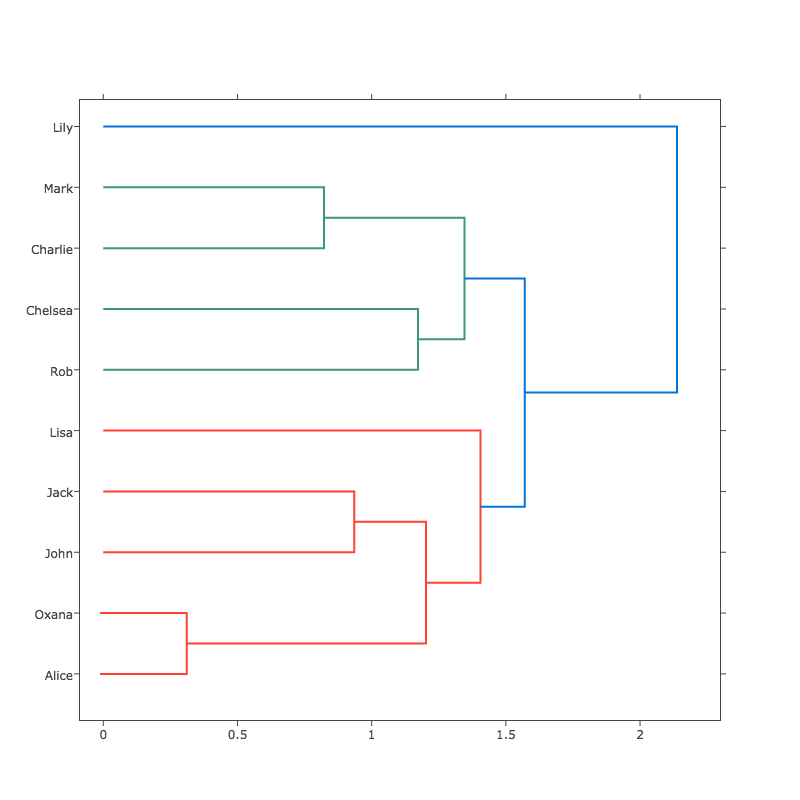
\includegraphics[width=\linewidth]{images/newplot}\\
    \end{center}
  \end{minipage}\\
  \makebox[\linewidth]{\hrulefill}
  \makebox[\linewidth]{\hrulefill}
  \makebox[\linewidth]{\hrulefill}

\end{document}
